\section{Исследование функций и уравнений решения}
1. По теореме Виета $x_1+x_2=10,\ x_1x_2=q.$ Тогда $x_1^2+x_2^2=(x_1+x_2)^2-2x_1x_2=100-2q=2\Rightarrow q=49.$ Дискриминант уравнения в этом случае равен -171, а значит корней нет и таких $q$ не существует.\\
2. По теореме Виета $x_1+x_2=6,\ x_1x_2=q.$ Тогда $x_1^2+x_2^2=(x_1+x_2)^2-2x_1x_2=36-2q=4\Rightarrow q=16.$ Дискриминант уравнения в этом случае равен -28, а значит корней нет и таких $q$ не существует.\\
3. Первое уравнение задаёт на плоскости прямую, а второе --- окружность. Они могут иметь 0, 1 или 2 точки пересечения.\\
4. Первое уравнение задаёт на плоскости прямую, а второе --- окружность. Они могут иметь 0, 1 или 2 точки пересечения.\\
5. Для нахождения области определения $f(x)$ необходимо решить неравенство\\ $\cfrac{x(x^2+x-12)(x^2-3x+2)}{(x^2-x-6)(-x+5)}\geqslant0
\Leftrightarrow \cfrac{x(x+4)(x-3)(x-2)(x-1)}{(x-3)(x+2)(-x+5)}\geqslant0.$ Решим его, применив метод интервалов:
$x\in[-4;-2)\cup[0;1]\cup[2;3)\cup(3;5).$
\begin{figure}[ht!]
\center{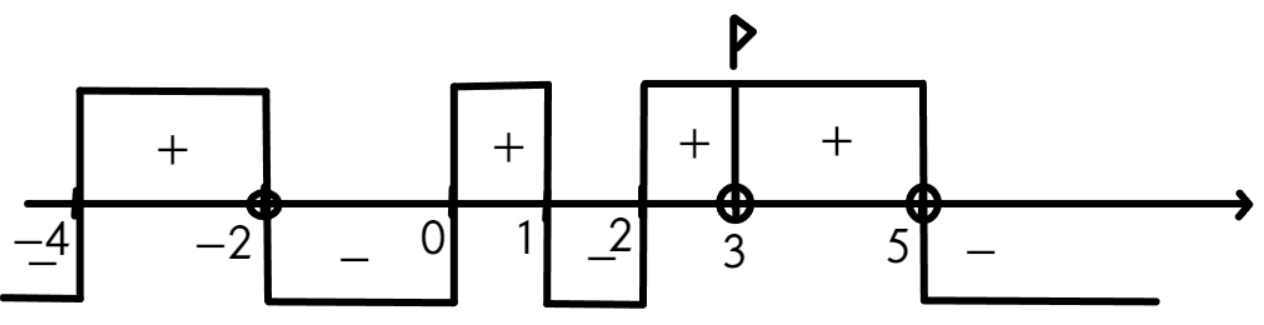
\includegraphics[scale=0.35]{isl9-5.png}}
\end{figure}\\
6. Для нахождения области определения $f(x)$ необходимо решить неравенство\\ $\cfrac{-x(x^2-2x-15)(x^2-6x+8)}{(x^2-11x+30)(x+1)}\geqslant0
\Leftrightarrow \cfrac{-x(x-5)(x+3)(x-2)(x-4)}{(x-5)(x+6)(x+1)}\geqslant0.$ Решим его, применив метод интервалов:
$x\in[-3;-1)\cup[0;2]\cup[4;5)\cup(5;6).$
\begin{figure}[ht!]
\center{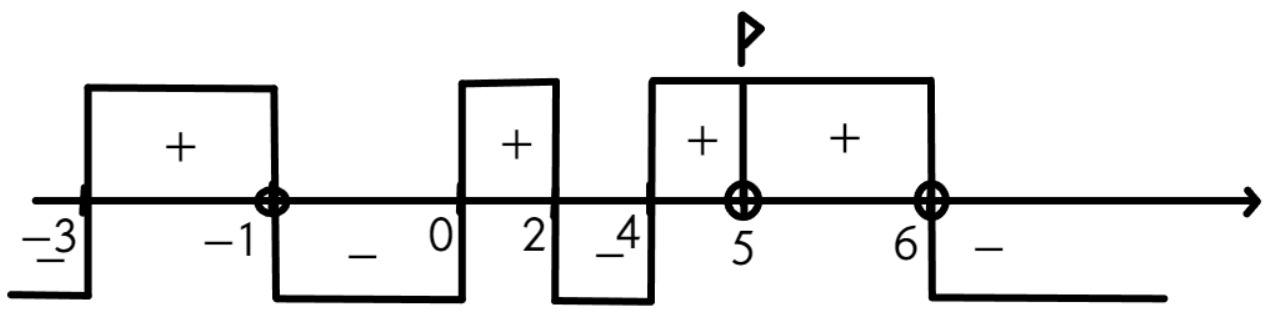
\includegraphics[scale=0.35]{isl9-6.png}}
\end{figure}\\
7. Если корнями уравнения являются числа $x_1$ и $x_2=x_1^2,$ то по теореме Виета имеем равенство $x_1\cdot x_1^2=x_1^3=a^3,$ откуда $x_1=a,\ x_2=a^2.$ По теореме Виета эти числа будут являться корнями уравнения тогда и только тогда, когда $a+a^2=\cfrac{15}{4},\ 4a^2+4a-15=0,\ a=\cfrac{3}{2}$ или $a=-\cfrac{5}{2}.$\\
8. Если корнями уравнения являются числа $x_1$ и $x_2=x_1^2,$ то по теореме Виета имеем равенство $x_1\cdot x_1^2=x_1^3=a^3,$ откуда $x_1=a,\ x_2=a^2.$ По теореме Виета эти числа будут являться корнями уравнения тогда и только тогда, когда $a+a^2=\cfrac{63}{4},\ 4a^2+4a-63=0,\ a=\cfrac{7}{2}$ или $a=-\cfrac{9}{2}.$\\
9. Для нахождения области определения $f(x)$ необходимо решить систему $\begin{cases} 4+3x-x^2>0,\\ x-2\neq0.\end{cases}\Leftrightarrow
\begin{cases} (x-4)(x+1)<0,\\ x\neq2.\end{cases}\Leftrightarrow x\in(-1;2)\cup(2;4).$\\
10. Для нахождения области определения $f(x)$ необходимо решить систему $\begin{cases} 3+2x-x^2>0,\\ x-1\neq0.\end{cases}\Leftrightarrow
\begin{cases} (x-3)(x+1)<0,\\ x\neq1.\end{cases}\Leftrightarrow x\in(-1;1)\cup(1;3).$\\
11. Пусть корни уравнения равны $a$ и $a+2,$ тогда по теореме Виета $a(a+2)=15,\ a^2+2a-15=0,\ a=3$ или $a=-5.$ То есть корнями могут быть числа 3 и 5 или $-5$ и $-3.$ По той же теореме Виета имеем равенство $3+5=k,$ то есть $k=8$ или $(-3)+(-5)=k,$ то есть $k=-8.$\\
12. Пусть корни уравнения равны $a$ и $a+2,$ тогда по теореме Виета $a(a+2)=3,\ a^2+2a-3=0,\ a=1$ или $a=-3.$ То есть корнями могут быть числа 1 и 3 или $-3$ и $-1.$ По той же теореме Виета имеем равенство $1+3=k,$ то есть $k=4$ или $(-1)+(-3)=k,$ то есть $k=-4.$\\
13. Уравнение имеет два различных корня, если $k\neq0$ и $D>0,$ то есть $(k+1)^2-4k(2k-1)=k^2+2k+1-8k^2+4k=-7k^2+6k+1>0,\ 7k^2-6k-1<0,\ (7k+1)(k-1)<0,\ k\in\left(-\cfrac{1}{7};1\right).$ Таким образом, $k\in\left(-\cfrac{1}{7};0\right)\cup(0;1).$\\
14. Уравнение имеет два различных корня, если $k\neq0$ и $D>0,$ то есть $(k-1)^2-4k(2k+1)=k^2-2k+1-8k^2-4k=-7k^2-6k+1>0,\ 7k^2+6k-1<0,\ (7k-1)(k+1)<0,\ k\in\left(-1;\cfrac{1}{7}\right).$ Таким образом, $k\in\left(-1;0\right)\cup\left(0;\cfrac{1}{7}\right).$\\
15. $y=-x+2\sqrt{x}-2=-((\sqrt{x})^2-2\sqrt{x}+1)-1=-(\sqrt{x}-1)^2-1\leqslant-1.$\\
16. $y=-x+4\sqrt{x}-5=-((\sqrt{x})^2-4\sqrt{x}+4)-1=-(\sqrt{x}-2)^2-1\leqslant-1.$\\
17. Пусть $t=2x-3,$ тогда $x=\cfrac{t+3}{2}$ и $f(t)=4\cdot\cfrac{t+3}{2}-5=2t+1$ Таким образом, $f(x)=2x+1.$\\
18. Пусть $t=2x+3,$ тогда $x=\cfrac{t-3}{2}$ и $f(t)=4\cdot\cfrac{t-3}{2}+5=2t-1$ Таким образом, $f(x)=2x-1.$\\
19. Уравнение имеет ровно один корень либо если $2a=0,\ a=0,$ либо если $D=(10-a)^2-8a(-a+5)=a^2-20a+100+8a^2-40a=9a^2-60a+100=(3a-10)^2=0,\ a=\cfrac{10}{3}.$\\
20. Уравнение имеет ровно один корень либо если $2a=0,\ a=0,$ либо если $D=(10+a)^2-8a(-a-5)=a^2+20a+100+8a^2+40a=9a^2+60a+100=(3a+10)^2=0,\ a=-\cfrac{10}{3}.$\\
21. По теореме Виета $x_1+x_2=\cfrac{3}{2},\ x_1x_2=-\cfrac{11}{2}.$ Тогда $\cfrac{x_2}{1+x_1}+\cfrac{x_1}{1+x_2}=\cfrac{x_2+x_2^2+x_1+x_1^2}{1+x_1+x_2+x_1x_2}=
\cfrac{(x_1+x_2)^2+x_1+x_2-2x_1x_2}{1+x_1+x_2+x_1x_2}=\cfrac{\cfrac{9}{4}+\cfrac{3}{2}+11}{1+\cfrac{3}{2}-\cfrac{11}{2}}=-\cfrac{59}{12}.$\\
22. По теореме Виета $x_1+x_2=-2,\ x_1x_2=-\cfrac{8}{9}.$ Тогда $x_1^3+x_2^3=(x_1+x_2)(x_1^2-x_1x_2+x_2^2)=(x_1+x_2)((x_1+x_2)^2-3x_1x_2)=(-2)\left(4+\cfrac{8}{3}\right)=-\cfrac{40}{3}.$\\
23. Корни уравнения лежат по разные стороны от 1 тогда и только тогда, когда выполняется неравенство $(x_1-1)(x_2-1)<0,\ x_1x_2-(x_1+x_2)+1<0.$ По теореме Виета имеем равенства $x_1+x_2=\cfrac{2a+1}{1-a^2},\ x_1x_2=\cfrac{3}{1-a^2}.$ Поэтому $\cfrac{3}{1-a^2}-\cfrac{2a+1}{1-a^2}+1<0,\
\cfrac{3-2a-a^2}{1-a^2}<0,\ \cfrac{(a+3)(a-1)}{(a-1)(a+1)}<0,\ a\in(-3;-1).$ Кроме того, необходимо проверить, что при этих значениях $a$ уравнение имеет два корня. Старший коэффициент обнуляется при $a=\pm1,$ которые в полученные интервал не входят. Остаётся проверить неравенство $D>0,$ то есть $(2a+1)^2+12(a^2-1)>0,$ что верно, так как квадрат всегда неотрицателен, а $a^2$ при полученных значениях $a$ больше 1.\\
24. Корни уравнения лежат по разные стороны от $(-1)$ тогда и только тогда, когда выполняется неравенство $(x_1+1)(x_2+1)<0,\ x_1x_2+(x_1+x_2)+1<0.$ По теореме Виета имеем равенства $x_1+x_2=\cfrac{3b-1}{4-b^2},\ x_1x_2=\cfrac{7}{4-b^2}.$ Поэтому $\cfrac{7}{4-b^2}+\cfrac{3b-1}{4-b^2}+1<0,\
\cfrac{10+3b-b^2}{4-b^2}<0,\ \cfrac{(b+2)(b-5)}{(b-2)(b+2)}<0,\ b\in(2;5).$ Кроме того, необходимо проверить, что при этих значениях $b$ уравнение имеет два корня. Старший коэффициент обнуляется при $b=\pm2,$ которые в полученные интервал не входят. Остаётся проверить неравенство $D>0,$ то есть $(3b-1)^2+28(b^2-4)>0,$ что верно, так как квадрат всегда неотрицателен, а $b^2$ при полученных значениях $b$ больше 4.\\
25. Наименьшее значение параболы достигается в вершине $x=-\cfrac{-6}{2}=3,$ значит $9-18+a=1,\ a=10.$\\
26. Наибольшее значение параболы достигается в вершине $x=-\cfrac{4}{-2}=2,$ значит $-4+8+a=2,\ a=-2.$\\
27. Парабола неотрицательна на отрезке, если её старший коэффициент отрицателен, и она имеет два корня. То есть необходимо решить систему неравенств $\begin{cases} a-3<0,\\ (a+1)^2-4(a-3)(a+1)>0.\end{cases}\Leftrightarrow\begin{cases} a<3,\\ a^2+2a+1-4a^2+8a+12>0.\end{cases}\Leftrightarrow
\begin{cases} a<3,\\ 3a^2-10a-13<0.\end{cases}\Leftrightarrow\begin{cases} a<3,\\ (a+1)(3a-13)<0.\end{cases}\Leftrightarrow$\\$
\begin{cases} a<3,\\ a\in\left(-1;\cfrac{13}{3}\right).\end{cases}\Leftrightarrow a\in(-1;3).$\\
28. Парабола неотрицательна на отрезке, если её старший коэффициент отрицателен, и она имеет два корня. То есть необходимо решить систему неравенств $\begin{cases} a+2<0,\\ (a-1)^2-4(a+2)(a-1)>0.\end{cases}\Leftrightarrow\begin{cases} a<-2,\\ a^2-2a+1-4a^2-4a+8>0.\end{cases}\Leftrightarrow
\begin{cases} a<-2,\\ 3a^2+6a-9<0.\end{cases}\Leftrightarrow\begin{cases} a<3,\\ 3(a-1)(a+3)<0.\end{cases}\Leftrightarrow$\\$
\begin{cases} a<-2,\\ a\in\left(-3;1\right).\end{cases}\Leftrightarrow a\in(-3;-2).$\\
29. Наибольшее значение достигается при $m=-3,\ n=2$ и равно $9-2=7.$ Наименьшее значение достигается при $m=-\cfrac{\sqrt{2}}{2},\ n=1,6$ и равно $\cfrac{1}{2}-\cfrac{5}{2}=-2.$\\
30. Наибольшее значение достигается при $a=-1,5,\ b=2,4$ и равно $2,4-0,9=1,5.$ Наименьшее значение достигается при $a=-5,\ b=-0,5$ и равно $-0,5-10=-10,5.$\\
31. Корни уравнения лежат по разные стороны от 2 тогда и только тогда, когда выполняется неравенство $(x_1-2)(x_2-2)<0,\ x_1x_2-2(x_1+x_2)+4<0.$ По теореме Виета имеем равенства $x_1+x_2=5-a,\ x_1x_2=a^2-a.$ Поэтому $a^2-a+2a-10+4<0,\
a^2+a-6<0,\ (a+3)(a-2)<0,\ a\in(-3;2).$ Кроме того, необходимо проверить, что при этих значениях $a$ уравнение имеет два корня. Для это рассмотрим неравенство $D>0,$ то есть $(a-5)^2-4(a^2-a)>0,\ a^2-10a+25-4a^2+4a>0,\ 3a^2+6a-25<0,\ 3(a+1)^2<28.$ При полученных ранее значениях $a$ это неравенство выполняется, так как максимальное значение левой части равно $3\cdot9=27<28.$\\
32. Корни уравнения лежат по разные стороны от $(-1)$ тогда и только тогда, когда выполняется неравенство $(x_1+1)(x_2+1)<0,\ x_1x_2+(x_1+x_2)+1<0.$ По теореме Виета имеем равенства $x_1+x_2=a-7,\ x_1x_2=a^2-6a.$ Поэтому $a^2-6a+a-7+1<0,\ a^2-5a-6<0,\ (a-6)(a+1)<0,\ a\in(-1;6).$ Кроме того, необходимо проверить, что при этих значениях $a$ уравнение имеет два корня. Для это рассмотрим неравенство $D>0,$ то есть $(a-7)^2-4(a^2-6a)>0,\ a^2-14a+49-4a^2+24a>0,\ 3a^2-10a-49<0,\ \left(a-\cfrac{5}{3}\right)^2<\cfrac{172}{9}.$ При полученных ранее значениях $a$ это неравенство выполняется, так как максимальное значение левой части равно $\left(6-\cfrac{5}{3}\right)^2=\cfrac{169}{9}<\cfrac{172}{9}.$\\
33. Решим неравенство: $1,6+13t-5t^2\geqslant4,\ 5t^2-12t+2,4\leqslant0,\ 5(t-2,4)(t-0,2)\leqslant0,\ t\in[0,2;2,4].$ Значит, мяч будет находиться на высоте не менее 4 метров в течение $2,4-0,2=2,2$с.\\
34. Решим неравенство: $1,4+9t-5t^2\geqslant3,\ 5t^2-9t+1,6\leqslant0,\ 5(t-1,6)(t-0,2)\leqslant0,\ t\in[0,2;1,6].$ Значит, мяч будет находиться на высоте не менее 3 метров в течение $1,6-0,2=1,4$с.\\
35. Корни квадратного уравнения расположены симметрично относительно вершины параболы, значит $-\cfrac{a^2+5a-2}{2a}=-2,\ a^2+5a-2=4a,\ a^2+a-2=0,\ a=-2$ или $a=1.$ Для найденных значений $a$ необходимо проверить количество корней. При $a=-2$ получаем уравнение $-2x^2+(4-10-2)x-2+4=0,\ 2x^2+8x-2=0,\ D>0.$ При $a=1$ получаем уравнение $x^2+(1+5-2)x+1+4=0,\ x^2+4x+5=0,\ D<0.$ Значит, подходит только $a=-2.$\\
36. Корни квадратного уравнения расположены симметрично относительно вершины параболы, значит $-\cfrac{a^2+a-2}{2a}=-1,\ a^2+a-2=2a,\ a^2-a-2=0,\ a=-1$ или $a=2.$ Для найденных значений $a$ необходимо проверить количество корней. При $a=-1$ получаем уравнение $-x^2+(1-1-2)x-1+4=0,\ x^2+2x-3=0,\ D>0.$ При $a=2$ получаем уравнение $2x^2+(4+2-2)x+2+4=0,\ 2x^2+4x+6=0,\ D<0.$ Значит, подходит только $a=-1.$\\
37. $y=7+\sqrt{x^2-2x+5}=7+\sqrt{(x-1)^2+4}\geqslant7+2=9.$\\
38. $y=6+\sqrt{3-x^2-2x}=6+\sqrt{4-(x+1)^2}\geqslant6+0=6.$\\
39. Уравнение $ax^2+(4a+2)x+3a+1,5=0$ имеет единственный корень либо если $a=0,$ либо если $\cfrac{D}{4}=0,\ (2a+1)^2-a(3a+1,5)=4a^2+4a+1-3a^2-1,5a=a^2+2,5a+1=0,\
a=-2$ или $a=-\cfrac{1}{2}.$\\
40. Уравнение $ax^2-(2a+6)x+3a+3=0$ имеет единственный корень либо если $a=0,$ либо если $\cfrac{D}{4}=0,\ (a+3)^2-a(3a+3)=a^2+6a+9-3a^2-3a=-2a^2+3a+9=0,\
a=3$ или $a=-\cfrac{3}{2}.$\\
41. $23-\cfrac{16}{x^2-2x+5}=23-\cfrac{16}{(x-1)^2+4}\geqslant23-\cfrac{16}{4}=19.$\\
42. $5+\cfrac{16}{x^2+2x+5}=5+\cfrac{16}{(x+1)^2+4}\geqslant5+\cfrac{16}{4}=9.$\\
43. Если $x-y=3,$ то $x=y+3.$ Тогда $x^2-4xy+y^2=(y+3)^2-4y(y+3)+y^2=y^2+6y+9-4y^2-12y+y^2=-2y^2-6y+9=-2(y^2+3y+2,25)+13,5=
-2(y+1,5)^2+13,5\leqslant13,5.$\\
44. Если $2x-y=1,$ то $y=2x-1.$ Тогда $5x^2+4xy-5y^2=5x^2+4x(2x-1)-5(2x-1)^2=5x^2+8x^2-4x-20x^2+20x-5=-7x^2+16x-5=-7\left(x^2-\cfrac{16}{7}x+\cfrac{64}{49}\right)+\cfrac{29}{7}=
-7\left(x-\cfrac{16}{7}\right)^2+\cfrac{29}{7}\leqslant\cfrac{29}{7}.$\\
45. $x^3+6x^2+ax=0,\ x(x^2+6x+a)=0.$ Это уравнение всегда имеет корень $x=0.$ Всего у уравнения два корня либо если один из корней уравнения $x^2+6x+a=0$ также равен нулю, либо если у него один (другой) корень. В первом случае $0+0+a=0,\ a=0,$ а во втором случае $\cfrac{D}{4}=9-a=0,\ a=9.$\\
46. $4x^3+4x^2+ax=0,\ x(4x^2+4x+a)=0.$ Это уравнение всегда имеет корень $x=0.$ Всего у уравнения два корня либо если один из корней уравнения $4x^2+4x+a=0$ также равен нулю, либо если у него один (другой) корень. В первом случае $0+0+a=0,\ a=0,$ а во втором случае $\cfrac{D}{4}=4-4a=0,\ a=1.$\\
47. $(\sqrt{19-a}+\sqrt{10-a})(\sqrt{19-a}-\sqrt{10-a})=19-a-(10-a)=9,$ значит $\sqrt{19-a}+\sqrt{10-a}=9:1=9.$\\
48. $(\sqrt{13-a}+\sqrt{6-a})(\sqrt{13-a}-\sqrt{6-a})=13-a-(6-a)=7,$ значит $\sqrt{13-a}+\sqrt{6-a}=7:1=7.$\\
49. Подставим $x=3$ и воспользуемся нечётностью функции, тогда $3f(2)+2f(-2)=2\cdot3+1,\ 3f(2)-2f(2)=7,\ f(2)=7.$\\
50. Подставим $x=5$ и воспользуемся нечётностью функции, тогда $2f(3)+5f(-3)=2\cdot5-1,\ 2f(3)-5f(3)=9,\ f(3)=-3.$\\
51. Пусть $f(x)=ax^2+bx+c,$ тогда получим систему уравнений $\begin{cases}a+b+c=1,\\ 9a+3b+c=27,\\ 16a+4b+c=64.\end{cases}$ Вычтем из второго уравнения первое, получим соотношение $8a+2b=26,\ b=13-4a.$ Вычтем из третьего уравнения первое и подставим вместо $b$ выражение $13-4a:\ 15a+3b=63,\ 5a+b=21,\ 5a+13-4a=21,\ a=8.$ Тогда $b=13-4\cdot8=-19,\ c=1-a-b=1-8+19=12.$ Таким образом, $f(x)=8x^2-19x+12.$\\
52. Пусть $f(x)=ax^2+bx+c,$ тогда получим систему уравнений $\begin{cases}a+b+c=1,\\ 4a+2b+c=8,\\ 16a+4b+c=64.\end{cases}$ Вычтем из второго уравнения первое, получим соотношение $3a+b=7,\ b=7-3a.$ Вычтем из третьего уравнения первое и подставим вместо $b$ выражение $7-3a:\ 15a+3b=63,\ 5a+b=21,\ 5a+7-3a=21,\ a=7.$ Тогда $b=7-3\cdot7=-14,\ c=1-a-b=1-7+14=8.$ Таким образом, $f(x)=7x^2-14x+8.$\\
53. Для нахождения области определения функции необходимо решить систему:\\ $\begin{cases} |x-1|(3x-6)\geqslant0,\\ x^2+4x-21\neq0.\end{cases}\Leftrightarrow
\begin{cases} \left[\begin{array}{l} x=1,\\ x\geqslant2.\end{array}\right.\\ x\neq-7,\ x\neq3.\end{cases}\Leftrightarrow x\in \{1\}\cup[2;3)\cup(3;+\infty).$\\
54. $y=\cfrac{(x+6)(x^3-27)}{x^2+3x-18}=\cfrac{(x+6)(x-3)(x^2+3x+9)}{(x+6)(x-3)}=x^2+3x+9,\ x\neq-6,\ x\neq3.$ Наименьшее значение парабола достигает в вершине $x_{\text{верш}}=-\cfrac{3}{2}$ и оно равно $\cfrac{9}{4}-\cfrac{9}{2}+9=\cfrac{27}{4}.$ При $x=-6$ и $x=3$ получим значения $36-18+9=27$ и $9+9+9=27.$ Значит, множество значений функции --- это $\left[\cfrac{27}{4};27\right)\cup(27;+\infty).$\\
55. Корни уравнения лежат по разные стороны от 1 тогда и только тогда, когда выполняется неравенство $(x_1-1)(x_2-1)<0,\ x_1x_2-(x_1+x_2)+1<0.$ По теореме Виета имеем равенства $x_1+x_2=2b+3,\ x_1x_2=-b-6.$ Поэтому $-b-6-2b-3+1<0,\
b>-\cfrac{8}{3}.$ Кроме того, необходимо проверить, что при этих значениях $b$ уравнение имеет два корня. Решим неравенство $D>0,$ то есть $(2b+3)^2+4(b+6)>0,\
4b^2+12b+9+4b+24>0,\ 4b^2+16b+33=(2b+4)^2+17>0.$ Оно выполняется при любых значениях $b,$ значит $b\in\left(-\cfrac{8}{3};+\infty\right).$\\
56. Решим данное уравнение графически. Правая часть представляет из себя гиперболу, а левая --- модуль, коэффициент при котором влияет на то, насколько большой угол при вершине $(5;0)$ будет образован.
$$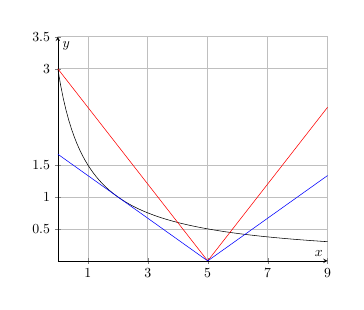
\begin{tikzpicture}[scale=0.5]
\begin{axis}[
    axis lines = middle,
    grid=major,
    legend pos={south west},
    xlabel = {$x$},
    %xlabel style={below right},
    ylabel = {$y$},
    ymax=3.5,
    xtick={1, 3, 5, 7, 9},
    xticklabels={1, 3, 5, 7, 9},
    ytick={0.5,1,1.5,3,3.5},
    yticklabels={0.5,1,1.5,3,3.5},
               ]
	\addplot[domain=0:9, samples=100, color=black] {3/(x+1)};
    \addplot[domain=0:9, samples=100, color=red] {0.6*abs(x-5)};
    \addplot[domain=0:9, samples=100, color=blue] {abs(x-5)/3};
	%\addlegendentry{$\text{Рис. 1}$};
\end{axis}
\end{tikzpicture}$$
Чем больше значение $a,$ тем меньше угол и, соответственно, выше точка пересечения с осью ординат. Гипербола пересекает её при $y=\cfrac{3}{0+1}=3.$ Найдём, при каком значении $a$ график модуля также пройдёт через эту точку: $a\cdot|0+1|=3,\ a=\cfrac{3}{5}.$ При $a>\cfrac{3}{5}$ гипербола будет иметь с модулем ровно две точки пересечения. При $a\leqslant\cfrac{3}{5}$ они будут иметь сначала 3 точки пересечения, затем 2 (в случае касания), затем 0. Найдём, при каком значении $a$ график модуля касается гиперболы. Это происходит при $x<5,$ значит уравнение $a\cdot(5-x)\cfrac{3}{x+1}$ должно иметь единственное решение, то есть $a(5-x)(x+1)=3,\
5ax+5a-ax^2-ax=3,\ ax^2-4ax+3-5a=0$ имеет единственное решение. При $a=0$ точек пересечения нет, значит $\cfrac{D}{4}=4a^2-3a+5a^2=9a\left(a-\cfrac{1}{3}\right)=0,$
откуда $a=\cfrac{1}{3}.$ Итого ответом является множество $\left\{\cfrac{1}{3}\right\}\cup\left(\cfrac{3}{5};+\infty\right).$\\
57. $a+\cfrac{1}{a}=-4,\ \left(a+\cfrac{1}{a}\right)^2=a^2+2+\cfrac{1}{a^2}=16,$ откуда $a^2+\cfrac{1}{a^2}=14.$ Тогда\\ $a^3+\cfrac{1}{a^3}=
\left(a+\cfrac{1}{a}\right)\left(a^2-1+\cfrac{1}{a^2}\right)=(-4)(14-1)=-52.$\\
58.$\begin{cases}
(k+2)x+3y=9+kx,\\
x+(k+4)y=2.
\end{cases}\Leftrightarrow\begin{cases}
2x+3y=9,\\
x+(k+4)y=2.
\end{cases}
$
Каждое из уравнений задаёт прямую на плоскости, причём эти прямые разные, так как уравнения не пропорциональны $(2:1\neq9:2),$ поэтому бесконечно много решений система иметь не может.\\
59. а) Уравнение имеет единственное решение при $a-1=0,\ a=1$ или при $\cfrac{D}{4}=4(a+1)^2-(a-1)(a-4)=4a^2+8a+4-a^2+a+4a-4=3a^2+13a=a(3a+13)=0,\ a\in\left\{-\cfrac{13}{3};0\right\}.$\\
б) При $a=2$ уравнение имеет вид $x^2+12x-2=0.$ По теореме Виета $x_1+x_2=-12,\ x_1x_2=-2,$ тогда $x_1^3+x_2^3=(x_1+x_2)(x_1^2-x_1x_2+x_2^2)=(x_1+x_2)((x_1+x_2)^2-3x_1x_2)=(-12)\cdot(144+6)=-1800.$\\
в) При $a=-2$ неравенство примет вид $-3x^2-4x-6\geqslant b.$ Так как ветви этой параболы направлены вниз, решением будет отрезок в том случае, если значение $b$ меньше значения в вершине. Вершина находится в точке $x_{\text{верш}}=-\cfrac{-4}{-6}=-\cfrac{2}{3},\ y_{\text{верш}}=-3\cdot\cfrac{4}{9}+4\cdot\cfrac{2}{3}-6=-\cfrac{14}{3}.$ Значит, ответом является множество $\left(-\infty;-\cfrac{14}{3}\right).$\\
60. Наименьшее значение выражение принимает в вершине $x_{\text{верш}}=-\cfrac{-6}{2}=3,\ y_{\text{верш}}=9-18+1=-8.$ Наибольшее значение оно примет в том конце отрезка, который находится дальше от вершины, то есть в 10: $100-60+1=41.$ Значит, выражение принимает все значения от $-8$ до 41.\\
61. $-x^4-2x^3-3x^2-2x+3=-(x^4+2x^3+3x^2+2x-3)=-((x^2+x+1)^2-4).$ Искомое выражение принимает наибольшее значение в том случае, когда $x^2+x+1$ принимает наименьшее значение. Это происходит при $x_{\text{верш}}=-\cfrac{1}{2}$ и оно равно $\cfrac{1}{4}-\cfrac{1}{2}+1=\cfrac{3}{4}.$ Тогда наибольшее значение искомого выражения равно $-\cfrac{9}{16}+4=\cfrac{55}{16}.$\\
62. По теореме Виета имеем соотношения $x_1+x_2=1,\ x_1x_2=\cfrac{q}{2},$ тогда $(x_1-x_2)^2=(x_1+x_2)^2-4x_1x_2=1-4\cdot\cfrac{q}{2}=1-2q=9,\ q=-4.$ При этом значении $q$ уравнение имеет вид $2x^2-2x-4=0,$ его дискриминант положителен, значит $q=-4$ является ответом.\\
63. По теореме Виета имеем соотношения $x_1+x_2=4,\ x_1x_2=\cfrac{q}{2},$ тогда $x_1^2+x_2^2=(x_1+x_2)^2-2x_1x_2=16-2\cdot\cfrac{q}{2}=16-q=16,\ q=0.$ При этом значении $q$ уравнение имеет вид $2x^2-8x=0,$ его дискриминант положителен, значит $q=0$ является ответом.\\
64. Корни уравнения лежат по разные стороны от 1 тогда и только тогда, когда выполняется неравенство $(x_1-1)(x_2-1)<0,\ x_1x_2-(x_1+x_2)+1<0.$ По теореме Виета имеем равенства $x_1+x_2=5-a,\ x_1x_2=a^2-a.$ Поэтому $a^2-a+a-5+1<0,\
a^2-4<0,\ (a+2)(a-2)<0,\ a\in(-2;2).$ Кроме того, необходимо проверить, что при этих значениях $a$ уравнение имеет два корня. Для это рассмотрим неравенство $D>0,$ то есть $(a-5)^2-4(a^2-a)>0,\ a^2-10a+25-4a^2+4a>0,\ 3a^2+6a-25<0,\ 3(a+1)^2<28.$ При полученных ранее значениях $a$ это неравенство выполняется, так как максимальное значение левой части равно $3\cdot9=27<28.$\\
65. Корни уравнения лежат по разные стороны от $1$ тогда и только тогда, когда выполняется неравенство $(x_1-1)(x_2-1)<0,\ x_1x_2-(x_1+x_2)+1<0.$ По теореме Виета имеем равенства $x_1+x_2=7-a,\ x_1x_2=a^2-6a.$ Поэтому $a^2-6a-7+a+1<0,\ a^2-5a-6<0,\ (a-6)(a+1)<0,\ a\in(-1;6).$ Кроме того, необходимо проверить, что при этих значениях $a$ уравнение имеет два корня. Для это рассмотрим неравенство $D>0,$ то есть $(7-a)^2-4(a^2-6a)>0,\ a^2-14a+49-4a^2+24a>0,\ 3a^2-10a-49<0,\ \left(a-\cfrac{5}{3}\right)^2<\cfrac{172}{9}.$ При полученных ранее значениях $a$ это неравенство выполняется, так как максимальное значение левой части равно $\left(6-\cfrac{5}{3}\right)^2=\cfrac{169}{9}<\cfrac{172}{9}.$\\
66. Корни уравнения лежат по разные стороны от $(-1)$ тогда и только тогда, когда выполняется неравенство $(x_1+1)(x_2+1)<0,\ x_1x_2+(x_1+x_2)+1<0.$ По теореме Виета имеем равенства $x_1+x_2=a-7,\ x_1x_2=a^2-6a+4.$ Поэтому $a^2-6a+4+a-7+1<0,\ a^2-5a-2<0,\ a\in\left(\cfrac{5-\sqrt{33}}{2};\cfrac{5+\sqrt{33}}{2}\right).$ Кроме того, необходимо проверить, что при этих значениях $a$ уравнение имеет два корня. Для это рассмотрим неравенство $D>0,$ то есть $(a-7)^2-4(a^2-6a+4)>0,\ a^2-14a+49-4a^2+24a-16>0,\ 3a^2-10a-33<0,\ a\in\left(\cfrac{5-2\sqrt{31}}{3};\cfrac{5+2\sqrt{31}}{3}\right).$ При полученных ранее значениях $a$ это неравенство выполняется, так как $\cfrac{5-2\sqrt{31}}{3}<\cfrac{5-\sqrt{33}}{2}<\cfrac{5+\sqrt{33}}{2}<\cfrac{5+2\sqrt{31}}{3}.$\\
67. $\sqrt{2+x-x^2}(x^2-(a+1)x+a)=0,\ \sqrt{(1+x)(2-x)}(x-1)(x-a)=0.$ У этого уравнения точно есть корни $-1,\ 1$ и 2 при любом значении $a.$ Также у него
может появиться четвёртый корень $x=a,$ если $a\notin\{-1;1;2\}$ и $a\in[-1;2].$ Таким образом, при $a\in(-1;1)\cup(1;2): 4$ корня, а при всех остальных --- 3.\\
68. $2x^2-|a^2-3|x=1\Leftrightarrow 2x^2-|a^2-3|x-1=0.$ Так как $D=4|a^2-3|^2+8>0$ при любых значениях $a,$ два корня у этого уравнения есть всегда. По теореме Виета имеем равенство $x_1+x_2=\cfrac{|a^2-3|}{2}.$ Тогда $\cfrac{|a^2-3|}{2}>a\Leftrightarrow |a^2-3|>2a \Leftrightarrow \left[\begin{array}{l} a^2-3>2a,\\ a^2-3<-2a.\end{array}\right.\Leftrightarrow \left[\begin{array}{l} (a-3)(a+1)>0,\\ (a+3)(a-1)<0.\end{array}\right.\Leftrightarrow a\in(-\infty;1)\cup(3;+\infty).$\\
69. Так как $D=4+16|a^2-5|>0$ при любых значениях $a,$ два корня у этого уравнения есть всегда. По теореме Виета имеем равенство $x_1x_2=\cfrac{-|a^2-5|}{4}.$ Тогда $\cfrac{-|a^2-5|}{4}<a\Leftrightarrow |a^2-5|>-4a \Leftrightarrow \left[\begin{array}{l} a^2-5>-4a,\\ a^2-5<4a.\end{array}\right.\Leftrightarrow \left[\begin{array}{l} (a-1)(a+5)>0,\\ (a+1)(a-5)<0.\end{array}\right.\Leftrightarrow a\in(-\infty;-5)\cup(-1;+\infty).$\\
70. Пусть $f(x)=-x^2+4x-2,\ g(x)=\sqrt{x-2}.$ График функции $f(x)$ представляет из себя параболу с вершиной в точке $x_{\text{верш}}=-\cfrac{4}{-2}=2,$ значит на луче $[2;+\infty)$ функция $f(x)$ убывает. Функция $g(x)$ определена на $[2;+\infty)$ и на всём этом множестве возрастает. При этом $f(2)=2,\ g(2)=0$ и $f(3)=g(3)=1.$ Значит, $m(x)=\begin{cases} f(x),\ x\in[2;3],\\ g(x),\ x\in(3;+\infty).\end{cases}$ Таким образом, наименьшее значение функция $m(x)$ принимает при $x=3$ и оно равно 1.\\
71. Пусть $f(x)=x^2+4x+2,\ g(x)=-\sqrt{x+2}.$ График функции $f(x)$ представляет из себя параболу с вершиной в точке $x_{\text{верш}}=-\cfrac{4}{2}=-2,$ значит на луче $[-2;+\infty)$ функция $f(x)$ возрастает. Функция $g(x)$ определена на $[-2;+\infty)$ и на всём этом множестве убывает. При этом $f(-2)=-2,\ g(-2)=0$ и $f(-1)=g(-1)=-1.$ Значит, $m(x)=\begin{cases} f(x),\ x\in[-2;-1],\\ g(x),\ x\in(-1;+\infty).\end{cases}$ Таким образом, наибольшее значение функция $m(x)$ принимает при $x=-1$ и оно равно $-1.$\\
72. а) Сначала проверим значение $a,$ при котором это уравнение линейно: при $a=0$ получим $3x+1=0,\ x=-\cfrac{1}{3},$ значит оно подходит. Для квадратного уравнения проверим наличие корней: $D\geqslant0,\ (a-3)^2-4a=a^2-6a+9-4a=a^2-10a+9=(a-1)(a-9)\geqslant0,\ a\in(-\infty;1]\cup[9;+\infty).$ То, что все корни отрицательны, равносильно тому, что отрицательна их сумма и положительно произведение. Тогда по теореме Виета имеем неравенства $\begin{cases} \cfrac{1}{a}>0,\\ \cfrac{a-3}{a}<0.\end{cases} \Leftrightarrow a\in (0;3).$ Таким образом, итоговым ответом будет $a\in[0;1].$\\
б) Квадратное уравнение имеет два различных корня, если $a\neq0$ и $D>0,$ то есть \\$\begin{cases}a\neq0,\\ (a-1)(a-9)>0.\end{cases}\Leftrightarrow a\in(-\infty;0)\cup(0;1)\cup(9;+\infty).$\\
в) Это уравнение имеет один корень, если у числителя один корень (не равный 2) или если один из двух корней числителя равен 2 (и отбрасывается по ОДЗ). Из предыдущих пунктов у числителя один корень при $a\in\{0; 1; 9\}.$ Подставим $x=2:\ 4a-2(a-3)+1=0,\ 4a-2a+6+1=0,\ a=-\cfrac{7}{2}.$ Таким образом, итоговый ответ $a\in \left\{-\cfrac{7}{2};0; 1; 9\right\}.$\\
73. \begin{figure}[ht!]
\center{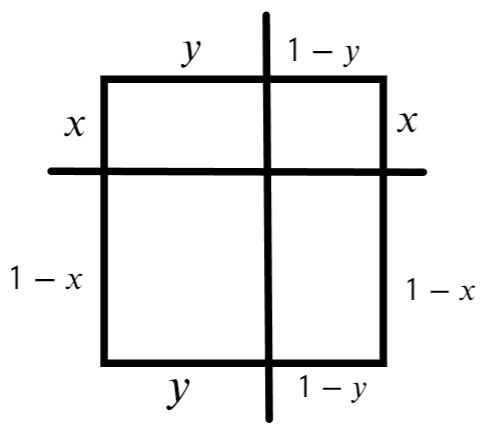
\includegraphics[scale=0.35]{issl9-73.png}}
\end{figure}\\
Обозначим сторону левого верхнего прямоугольника буквами $x$ и $y.$ Тогда произведение площадей равно $xy(1-x)(1-y)=(x-x^2)(y-y^2).$ График квадратичной функции $x-x^2$ представляет из себя параболу, ветви которой направлены вниз, а значит максимальное значение достигается в вершине, то есть при $x=-\cfrac{-1}{-2}=\cfrac{1}{2}.$ Оно равно $\cfrac{1}{2}-\cfrac{1}{4}=\cfrac{1}{4}.$ Второй множитель --- такая же функция, поэтому $S\leqslant \cfrac{1}{4}\cdot \cfrac{1}{4}=\cfrac{1}{16},$ ч.т.д.\\
74. Пусть $y=2x+1,$ тогда $x=\cfrac{y-1}{2}$ и $f(y)=4\cdot\cfrac{y^2-2y+1}{4}+1=y^2-2y+2,$ значит $f(x)=x^2-2x+2.$ График этой функции представляет из себя параболу с ветвями вверх, значит наибольшее значение достигается на одном из концов отрезка. Так как $f(0)=f(2)=2,$ оно равно 2.\\
75. Не умаляя общности пусть $a>b,$ тогда имеем систему уравнений $\begin{cases} a-b=41,\\ a+b=\sqrt{2022}.\end{cases}\Leftrightarrow$\\$ \begin{cases} 2a=\sqrt{2022}+41,\\ b=\sqrt{2022}-a.\end{cases}\Leftrightarrow\begin{cases} a=\cfrac{\sqrt{2022}+41}{2},\\ b=\cfrac{\sqrt{2022}-41}{2}.\end{cases}$ В таком случае $ab=\cfrac{\sqrt{2022}+41}{2}\cdot\cfrac{\sqrt{2022}-41}{2}=\cfrac{2022-1681}{4}=\cfrac{341}{4}.$\\
76. Выразим $x$ через $y:\ y^2x-y^2+4xy+6x-2y=3,\ x(y^2+4y+6)=y^2+2y+3,\ x=\cfrac{y^2+2y+3}{y^2+4y+6}.$ Числитель и знаменатель получившейся дроби всегда положительны, поэтому найти её минимальное значение --- это то же, что найти максимальное значение обратной дроби $\cfrac{y^2+4y+6}{y^2+2y+3}=1+\cfrac{2y+3}{y^2+2y+3}.$ Второе слагаемое не превосходит 1, так как $2y+3\leqslant y^2+2y+3,$ причём равенство достигается при $y^2=0,$ то есть $y=0.$ Значит, наибольшее значение обратной дроби равно 2, а наименьшее значение $x$ равно $\cfrac{1}{2}$ и достигается оно в паре $\left(\cfrac{1}{2};0\right).$\\
77. $y=(a+1)x^2+(5a-3)x+4a-5=ax^2+x^2+5ax-3x+4a-5=a(x^2+5x+4)+x^2-3x-5=a(x+4)(x+1)+x^2-3x-5.$ Чтобы точка была фиксированной, необходимо, чтобы $a$ сократилось, для этого достаточно взять $x=-4$ и $x=-1.$ В первом случае $y=16+12-5=23,$ а во втором --- $y=1+3-5=-1.$ Значит, графики этих функций всегда проходят через точки $(-4;23)$ и $(-1;-1),$ ч.т.д.\\
78. $\cfrac{x^2-3x+3}{1-x}=\cfrac{x^2+3(1-x)}{1-x}=\cfrac{x^2}{1-x}+3\geqslant3$ при $x<1.$ Значение 3 достигается при $x=0,$ знаит оно является наименьшим возможным значением дроби.\\
79. Так как $f(0)=c=3,$ по теореме Виета получим равенство $2,5\cdot x_2=\cfrac{3}{2},$ откуда второй корень $x_2=\cfrac{3}{2}\cdot\cfrac{2}{5}=\cfrac{3}{5}.$\\
80. У двух функций значение в 0 равно 0, а у третьей --- нет, значит ответы А и Б не подходят. Ответ Г не подходит, так как у каждой из функций есть нулевое значение, а его не может быть в знаменателе. Одна из функций положительна на рассматриваемом отрезке, а две других отрицательны. Если $f$ и $g$ обе отрицательны на отрезке, то значение их произведения на правом конце отрезка должно быть равно 0, что не выполняется. Значит, одна из них положительна, другая отрицательна, тогда отрицательно и их произведение, поэтому правильный ответ --- В.\\
81. $(\sqrt{x}-2)(ax+2)(3x-2a)=0\Leftrightarrow\begin{cases} \left[\begin{array}{l}x=-\cfrac{2}{a},\\ x=\cfrac{2a}{3},\\ x=4.\end{array}\right.\\ x\geqslant0.\end{cases}$ Один корень $x=4$ у этого уравнения есть всегда, значит из двух оставшихся должен подходить ровно один, или они должны совпадать друг с другом или с 4. Знаки этих корней всегда разные, значит подходить оба они никогда не могут. Если $-\cfrac{2}{a}=4,$ то $a=-\cfrac{1}{2}$ и у уравнения только один корень. Если $\cfrac{2a}{3}=4,$ то $a=6$ и у уравнения также только один корень. Совпадать друг с другом корни не могут, так как имеют разный знак, если $a=0,$ то один корень не существует, но другой подходит. Значит, это уравнение имеет два корня при $a\notin\left\{-\cfrac{1}{2};6\right\}.$\\
82. а) $$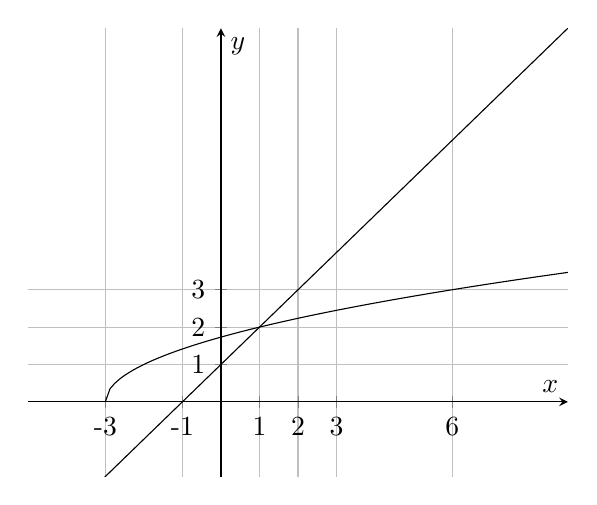
\begin{tikzpicture}[scale=1]
\begin{axis}[
    axis lines = middle,
    grid=major,
    legend pos={south west},
    xlabel = {$x$},
    %xlabel style={below right},
    ylabel = {$y$},
    ymin=-2,
    ymax=10,
    xmin=-5,
    xmax=9,
    xtick={-3,-1,1,2,3,6},
    xticklabels={-3,-1,1,2,3,6},
    ytick={3,2, 1},
    yticklabels={3,2, 1},
                  ]
	\addplot[domain=-3:9, samples=100, color=black] {sqrt(x+3)};
    \addplot[domain=-9:9, samples=100, color=black] {1+x};
        %\addplot[domain=2.01:6, samples=100, color=black] {2/(2-x)};
   % \addplot[domain=-3:3, samples=100, color=black] {-x};
     %\addlegendentry{$\text{Рис. 1}$};
\end{axis}
\end{tikzpicture}$$
По графику найдём ответ: $x\in[-3;1).$\\
б) Прямая $y=1+ax$ всегда проходит через точку $(0;1),$ и изменение параметра $a$ отвечает за её кручение вокруг этой точки. Если $a\leqslant0,$ то она пересечёт график $y=\sqrt{x+3}$ ровно один раз в левой полуплоскости. Если же $a>0,$ то она будет пересекать график два раза до тех пор, пока не пройдёт через точку $(-3;0),$ что произойдёт, когда $1-3a=0,\ a=\cfrac{1}{3}.$ При дальнейшем увеличении параметра $a$ прямая будет пересекать график только один раз в правой полуплоскости. Таким образом, $a\in(-\infty;0]\cup\left(\cfrac{1}{3};+\infty\right):$ 1 решение, $a\in\left(0;\cfrac{1}{3}\right]:$ 2 решения.\\
83.  Раз $|y|=x(2-x),$ должно выполняться неравенство $x(2-x)\geqslant0,$ поэтому $x\in[0;2].$ При этом $y=2x-x^2$ или $y=x^2-2x,$ а значит $x+y=3x-x^2$ или $x+y=x^2-x.$ У первой параболы вершина в точке $x=\cfrac{3}{2},$ значение в ней равно $\cfrac{9}{4}.$ Её наименьшее значение достигается на левом конце отрезка при $x=0$ и оно также равно 0. У второй параболы вершина в точке $x=\cfrac{1}{2},$ значение в ней равно $-\cfrac{1}{4}.$ Её наибольшее значение достигается на правом конце отрезка при $x=2$ и оно равно 2. Таким образом, выражение $x+y$ может принимать значения от $-\cfrac{1}{4}$ до $\cfrac{9}{4}.$\\
84. Применив теорему Виета, выразим $x_1^2+x_2^2=(x_1+x_2)^2-2x_1x_2=(-3)^2-2a=9-2a.$ Это значение уменьшается с ростом значения параметра $a,$ так что единственным ограничением является существование вещественных корней. Напишем неравенство для дискриминанта: $D=9-4a\geqslant0,$ значит $a\leqslant \cfrac{9}{4}.$ При этом значении $a$ корень будет только один, $x=-\cfrac{3}{2},$ а его квадрат равен $\cfrac{9}{4}.$\\
85. По теореме Виета $x_1+x_2=2,\ x_1x_2=q,$ тогда $x_1^2+x_2^2=(x_1+x_2)^2-2x_1x_2=4-2q=10084,$ поэтому $q=(4-10084):2=-5040.$ Найдём корни по формуле для квадратных уравнений с чётным вторым коэффициентом: $x=1\pm\sqrt{1+5041}=1\pm71=-70$ или 72.\\
86. По теореме Виета $x_1+x_2=3,\ x_1x_2=q,$ тогда $x_1^2+x_2^2=(x_1+x_2)^2-2x_1x_2=9-2q=2249,$ поэтому $q=(9-2249):2=-1120.$ Найдём корни по формуле : $x=\cfrac{3\pm\sqrt{9+4\cdot1120}}{2}=\cfrac{3\pm67}{2}=-32$ или 35.\\
87. Расстояния до осей координат от точки с координатами $(x,\ y)$ равны $|x|$ и $|y|,$ а значит требуется решить уравнение $|x|=|\sqrt{x^2+10x+34}+x-3|.$ Тогда $|x|=|\sqrt{x^2+10x+34}+x-3|\Leftrightarrow \left[\begin{array}{l} x=\sqrt{x^2+10x+34}+x-3,\\ x=3-x-\sqrt{x^2+10x+34}.\end{array}\right.\Leftrightarrow \left[\begin{array}{l} \sqrt{x^2+10x+34}=3-2x,\\ \sqrt{x^2+10x+34}=3.\end{array}\right.\Leftrightarrow$\\$ \left[\begin{array}{l} \begin{cases} x^2+10x+34=9-12x+4x^2,\\ 3-2x\geqslant0.\end{cases}\\ x^2+10x+34=9.\end{array}\right.\Leftrightarrow \left[\begin{array}{l} \begin{cases} 3x^2-22x-25=0,\\ x\leqslant\cfrac{3}{2}.\end{cases}\\ (x+5)^2=0.\end{array}\right.\Leftrightarrow \left[\begin{array}{l} \begin{cases} \left[\begin{array}{l} x=-1,\\ x=\cfrac{25}{3}.\end{array}\right.\\ x\leqslant\cfrac{3}{2}.\end{cases}\\ x=-5.\end{array}\right.\Leftrightarrow x\in\left\{-5;-1\right\}.$
Найдём теперь $f(-5)=\sqrt{25-50+34}-5-3=-5$ и $f\left(-1\right)=\sqrt{1-10+34}-1-3=1.$
Таким образом, подходят точки $(-5; -5)$ и $\left(-1;1\right).$\\
88. Расстояния до осей координат от точки с координатами $(x,\ y)$ равны $|x|$ и $|y|,$ а значит требуется решить уравнение $|x|=|\sqrt{x^2+4x+8}-x-2|.$ Тогда $|x|=|\sqrt{x^2+4x+8}-x-2|\Leftrightarrow \left[\begin{array}{l} x=\sqrt{x^2+4x+8}-x-2,\\ x=x+2-\sqrt{x^2+4x+8}.\end{array}\right.\Leftrightarrow \left[\begin{array}{l} \sqrt{x^2+4x+8}=2x+2,\\ \sqrt{x^2+4x+8}=2.\end{array}\right.\Leftrightarrow \left[\begin{array}{l} \begin{cases} x^2+4x+8=4x^2+8x+4,\\ 2x+2\geqslant0.\end{cases}\\ x^2+4x+8=4.\end{array}\right.\Leftrightarrow \left[\begin{array}{l} \begin{cases} 3x^2+4x-4=0,\\ x\geqslant-1.\end{cases}\\ (x+2)^2=0.\end{array}\right.\Leftrightarrow \left[\begin{array}{l} \begin{cases} \left[\begin{array}{l} x=-2,\\ x=\cfrac{2}{3}.\end{array}\right.\\ x\geqslant-1.\end{cases}\\ x=-2.\end{array}\right.\Leftrightarrow x\in\left\{-2;\cfrac{2}{3}\right\}.$
Найдём теперь f(-2)=$\sqrt{4-8+8}+2-2=2$ и $f\left(\cfrac{2}{3}\right)=\sqrt{\cfrac{4}{9}+\cfrac{8}{3}+8}-\cfrac{2}{3}-2=\cfrac{2}{3}.$
Таким образом, подходят точки $(-2; 2)$ и $\left(\cfrac{2}{3};\cfrac{2}{3}\right).$\\
89. Пусть уравнение этой прямой имеет вид $y=kx+b,$ тогда $10k+b=0,\ kx_1+b=x_1^2,\ kx_2+b=x_2^2,$ откуда $b=-10k$ и $x_1^2-x_2^2=k(x_1-x_2),\
(x_1-x_2)(x_1+x_2)=k(x_1-x_2),\ x_1+x_2=k,$ так как точки различны.
 Сложив второе и третье равенство, получим соотношение $k(x_1+x_2)+2b=x_1^2+x_2^2,\ k^2+2b=(x_1+x_2)^2-2x_1x_2,\ k^2+2b=k^2-2x_1x_2,\ x_1x_2=-b.$ Таким образом, $\cfrac{1}{x_1}+\cfrac{1}{x_2}=\cfrac{x_1+x_2}{x_1x_2}=\cfrac{k}{-b}=\cfrac{k}{10k}=\cfrac{1}{10}.$\\
90. То, что один корень лежит внутри отрезка, а другой вне, равносильно тому, что значения $f(x)$ на концах этого отрезка имеют разные знаки, поэтому $f(0)f(1)=b(1+a+b)<0.$ Таким образом, $f(b)=b^2+ab+b=b(b+a+1)<0.$\\
91. $(x-a)(x-10)+1=x^2-10x-ax+10a+1=x^2-(a+10)x+10a+1.$ У этого квадратного уравнения должны быть целые корни $-b$ и $-c,$ а значит его дискриминант является точным квадратом: $(a+10)^2-4(10a+1)=d^2,\ a^2+20a+100-40a-4-d^2=0,\
a^2-20a+100-d^2=4,\ (a-10)^2-d^2=4,\ (a-10-d)(a-10+d)=4.$ Заметим, что у чисел $a-10-d$ и $a-10+d$ одинаковая чётность, поэтому возможны два случая: $\begin{cases} a-10-d=2,\\ a-10+d=2. \end{cases}\Leftrightarrow \begin{cases} 2a-20=4,\\ a-10+d=2. \end{cases}\Leftrightarrow \begin{cases} a=12,\\ d=0.\end{cases}$ или
$\begin{cases} a-10-d=-2,\\ a-10+d=-2. \end{cases}\Leftrightarrow \begin{cases} 2a-20=-4,\\ a-10+d=-2. \end{cases}\Leftrightarrow \begin{cases} a=8,\\ d=0.\end{cases}$
Найденные значения $a$ надо подставить в исходное выражение и убедиться, что числа $b$ и $c$ получатся не только рациональными, но и целыми:
$(x-12)(x-10)+1=x^2-22x+120+1=(x-11)(x-11),\ (x-8)(x-10)+1=x^2-18x+80+1=(x-9)(x-9).$ Значит, оба полученных значения $a$ подходят.\\
92. $f(2x)=\cfrac{x+1}{2x+3}.$ Пусть $y=2x,$ тогда $x=\cfrac{y}{2}$ и $f(y)=\cfrac{\cfrac{y}{2}+1}{y+3}=\cfrac{y+2}{2y+6},$ а значит и
$f(x)=\cfrac{x+2}{2x+6}.$ Значит, необходимо решить уравнение
$\cfrac{x+2}{2x+6}-1=\cfrac{x+2-2x-6}{2x+6}=\cfrac{-x-4}{2x+6}=0,$ откуда $x=-4.$\\
93. Пусть $y=x+\cfrac{a}{x},$ тогда $y^2=\left(x+\cfrac{a}{x}\right)^2=
x^2+2x\cdot\cfrac{a}{x}+\cfrac{a^2}{x^2}=x^2+\cfrac{a^2}{x^2}+2a.$ Таким образом, $x^2+\cfrac{a^2}{x^2}-4\left(x+\cfrac{a}{x}\right)+10=
y^2-2a-4y+10=(y-2)^2+6-2a.$ Это выражение является полным квадратом, когда
$6-2a=0,\ a=3.$\\
94. $\cfrac{3x}{x^2+5x+9}=a \Leftrightarrow 3x=ax^2+5ax+9a
\Leftrightarrow ax^2+(5a-3)x+9a=0.$ Равносильности верны, так как знаменатель исходной дроби всегда положителен. По теореме Виета произведение корней получившегося уравнения равно $\cfrac{9a}{a}=9,$ значит единственное, что необходимо проверить --- это их существование. Запишем неравенство
$D=(5a-3)^2-4\cdot a\cdot9a> 0,\ 25a^2-30a+9-36a^2>0,\
11a^2+30a-9< 0,\ (a+3)(11a-3)< 0,\ a\in\left(-3;\cfrac{3}{11}\right).$
\newpage
